% Muestreo estratificado de 220 lotes para la revisión experta (sección 3.3.4).
% Las alturas son proporcionales al número de lotes de cada estrato (8 cm = total).
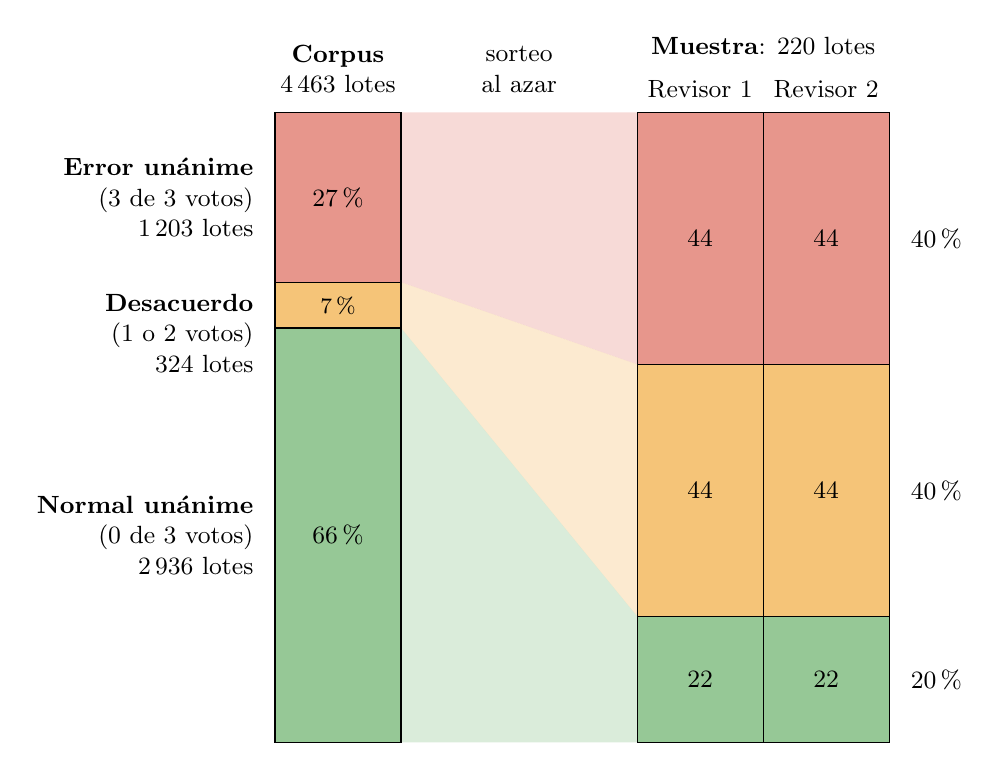
\begin{tikzpicture}[font=\small\linespread{1}\selectfont]
  \definecolor{eu}{RGB}{231,150,140}
  \definecolor{de}{RGB}{245,196,120}
  \definecolor{nu}{RGB}{150,200,150}

  % --- Conectores (sorteo), dibujados primero para quedar detrás de las barras
  \fill[eu, opacity=0.35] (1.6,8) -- (4.6,8) -- (4.6,4.8) -- (1.6,5.844) -- cycle;
  \fill[de, opacity=0.35] (1.6,5.844) -- (4.6,4.8) -- (4.6,1.6) -- (1.6,5.263) -- cycle;
  \fill[nu, opacity=0.35] (1.6,5.263) -- (4.6,1.6) -- (4.6,0) -- (1.6,0) -- cycle;

  % --- Corpus: 4 463 lotes
  \filldraw[fill=eu, draw=black] (0,5.844) rectangle (1.6,8);
  \filldraw[fill=de, draw=black] (0,5.263) rectangle (1.6,5.844);
  \filldraw[fill=nu, draw=black] (0,0)     rectangle (1.6,5.263);
  \node at (0.8,6.92) {27\,\%};
  \node at (0.8,5.55) {\footnotesize 7\,\%};
  \node at (0.8,2.63) {66\,\%};

  \node[anchor=east, align=right] at (-0.15,6.92) {\textbf{Error unánime}\\(3 de 3 votos)\\1\,203 lotes};
  \node[anchor=east, align=right] at (-0.15,5.20) {\textbf{Desacuerdo}\\(1 o 2 votos)\\324 lotes};
  \node[anchor=east, align=right] at (-0.15,2.63) {\textbf{Normal unánime}\\(0 de 3 votos)\\2\,936 lotes};

  % --- Muestra: 220 lotes, dividida en dos mitades sin solapamiento
  \foreach \x in {4.6,6.2} {
    \filldraw[fill=eu, draw=black] (\x,4.8) rectangle ++(1.6,3.2);
    \filldraw[fill=de, draw=black] (\x,1.6) rectangle ++(1.6,3.2);
    \filldraw[fill=nu, draw=black] (\x,0)   rectangle ++(1.6,1.6);
    \node at (\x+0.8,6.4) {44};
    \node at (\x+0.8,3.2) {44};
    \node at (\x+0.8,0.8) {22};
  }
  \node[anchor=west] at (7.95,6.4) {40\,\%};
  \node[anchor=west] at (7.95,3.2) {40\,\%};
  \node[anchor=west] at (7.95,0.8) {20\,\%};

  % --- Encabezados
  \node[align=center] at (0.8,8.55) {\textbf{Corpus}\\4\,463 lotes};
  \node[align=center] at (3.1,8.55) {sorteo\\al azar};
  \node at (6.2,8.85) {\textbf{Muestra}: 220 lotes};
  \node at (5.4,8.3) {Revisor 1};
  \node at (7.0,8.3) {Revisor 2};
\end{tikzpicture}
